% !TeX root = ../seminar.tex
\section{Isolated Black Holes}

{\setbeamercolor{background canvas}{bg=black}
\begin{frame}[plain]
\begin{tikzpicture}[remember picture, overlay]
  \node[inner sep=0] at (current page.center) {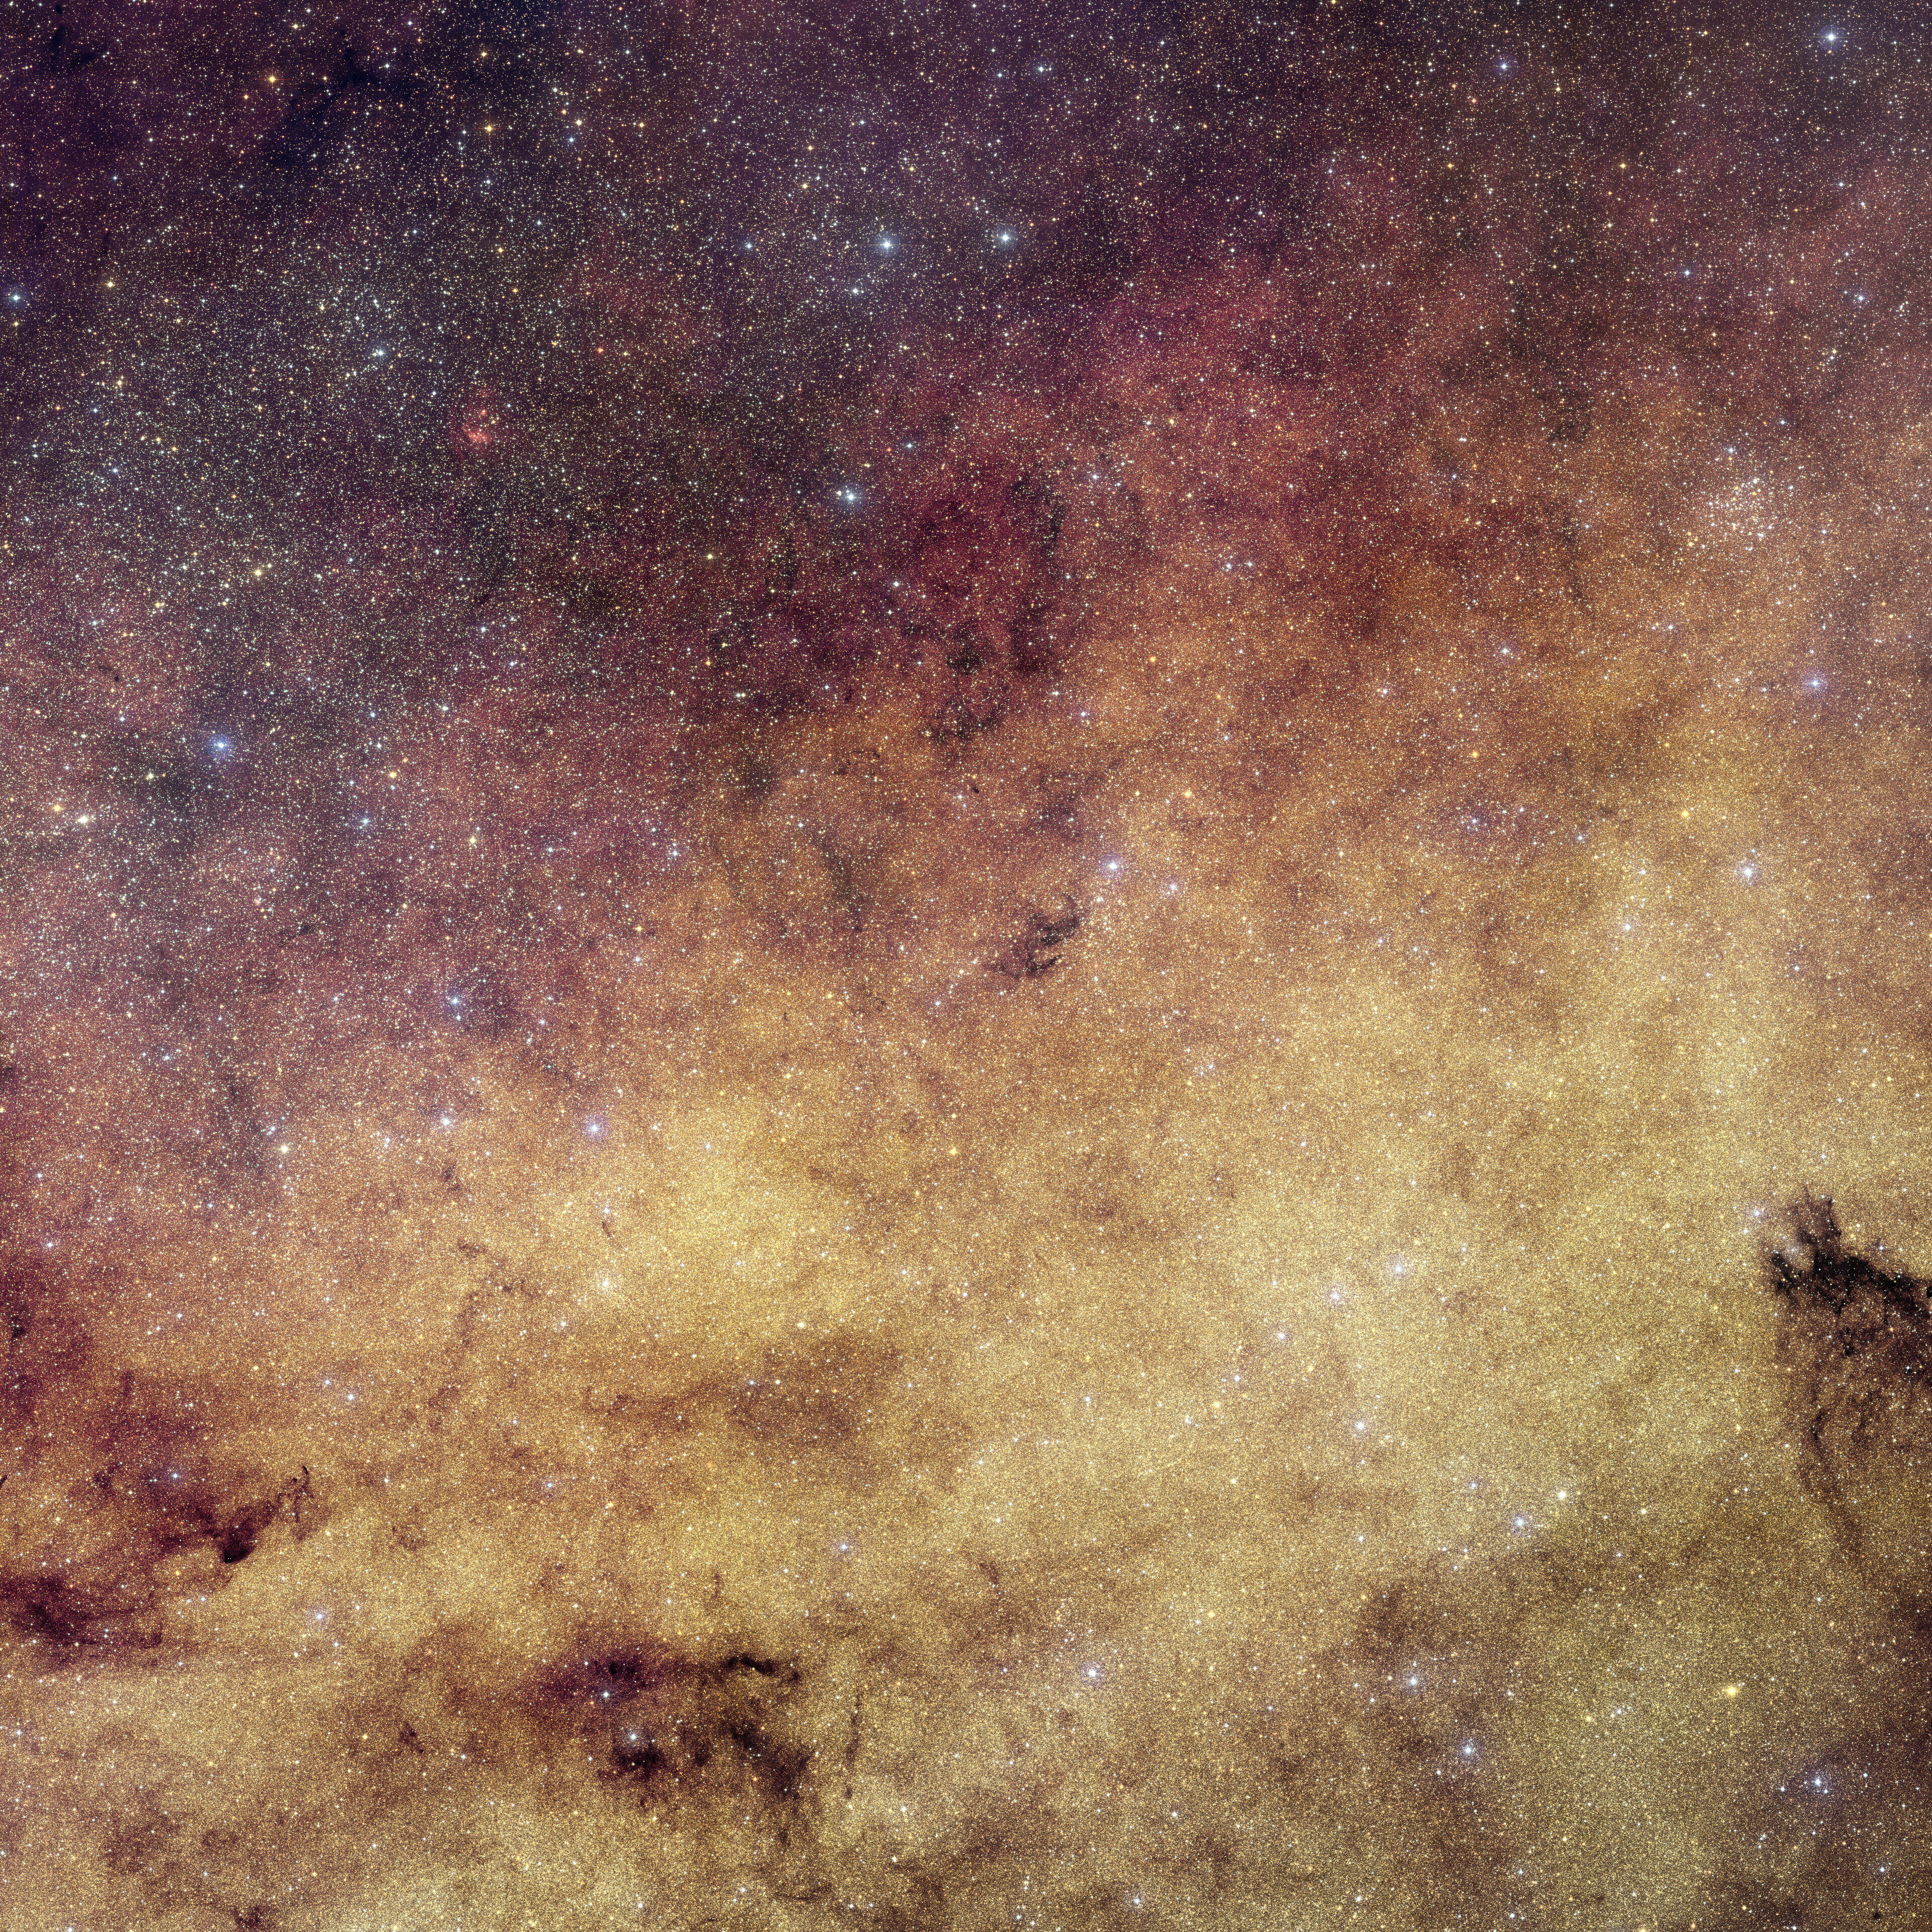
\includegraphics[width=\paperwidth]{euclid_bulge}};
  \node[bleedtitle, anchor=north west] at ([xshift=5mm, yshift=-4mm]current page.north west)
       {Black holes hide among these stars};
  \node[bleedtext, anchor=north west] at ([xshift=5mm, yshift=-15mm]current page.north west)
       {None of them shine};
  \bleedcredit{\href{https://www.nasa.gov/missions/roman-space-telescope/euclid-view-of-milky-way-heart-previews-core-survey-by-nasas-roman/}{ESA/Euclid/Euclid Consortium/NASA, CFHT; image processing J.-C.~Cuillandre \& E.~Bertin (CEA Paris-Saclay)}}
  \bleedsection
\end{tikzpicture}
\note{\begin{itemize}
  \item \emph{Euclid} with ground-based colour: a region near the Galactic centre that Roman's bulge survey will
        observe repeatedly.
  \item The Milky Way should hold $\sim10^8$ stellar black holes, and a field like this one hides many of them.
        Without a companion they emit nothing: the question of the next slides is how to find them.
\end{itemize}}
\end{frame}}


\begin{frame}{Almost every known black hole is in a binary}
\vspace{1mm}
$\sim\!10^8$ stellar black holes in the Milky Way; the known ones are seen through a \textbf{companion}\\
{\small (its light, X-rays from accretion, gravitational waves)}. \uncover<2->{Why not use those?}
\vspace{3mm}

\begin{columns}[T]
\begin{column}{.48\linewidth}
\textbf{In a binary}
\begin{itemize}\setlength{\itemsep}{5pt}
  \item<3-> \textbf{Mass} reshaped by the companion\\ {\small (mass transfer, stripped envelopes)}
  \item<4-> Only \textbf{weak kicks} survive\\ {\small (a strong kick unbinds the pair)}
  \item<5-> Seen only while \textbf{active}\\ {\small (X-ray outbursts: selection effects)}
\end{itemize}
\end{column}
\begin{column}{.48\linewidth}
\textbf{Isolated}
\begin{itemize}\setlength{\itemsep}{5pt}
  \item<3-> Mass set by the \textbf{star's own collapse}
  \item<4-> Carry their \textbf{full natal kick}
  \item<5-> Found by \textbf{gravity alone}:\\ every one can lens
\end{itemize}
\end{column}
\end{columns}
\vfill
\uncover<6->{%
\begin{beamercolorbox}[rounded=true,sep=6pt,wd=\linewidth]{block body alerted}
\centering
Binaries are not \emph{wrong}: they answer a different question (binary evolution).\\
Supernova physics and the Galaxy's black-hole census need the \textbf{isolated} ones too
\end{beamercolorbox}}
\vfill
\refnote{%
\ads{2020A\%26A...638A..94O}{Olejak et al.\ 2020};
\ads{2023MNRAS.518.1057E}{El-Badry et al.\ 2023};
\ads{2024A\%26A...686L...2G}{Gaia Collaboration 2024};
\ads{2012Sci...337..444S}{Sana et al.\ 2012, Science 337, 444};
\ads{2012MNRAS.425.2799R}{Repetto et al.\ 2012, MNRAS 425, 2799};
\ads{2012ApJ...757...36K}{Kreidberg et al.\ 2012, ApJ 757, 36}}
\note{\begin{itemize}
  \item Stars above $\sim20\,\Msun$ end as black holes. Population syntheses: $1.2\times10^8$ at $\sim14\,\Msun$
        (Olejak et al.\ 2020), $2.2\times10^8$ at $5$--$16\,\Msun$ (Lam et al.\ 2020).
  \item Known ones: X-ray binaries (accretion from a companion), \emph{Gaia} BH1--3 (a companion's orbit),
        gravitational-wave mergers (distant galaxies).
  \item Most massive stars are born in binaries that interact (Sana et al.\ 2012): the companion strips or feeds the
        progenitor, so a binary black hole's mass records binary evolution, not single-star collapse alone.
  \item Kicks: a black hole kicked hard enough leaves its companion and becomes isolated. Binaries keep the
        weak-kick ones, so their velocities underestimate the kicks (Repetto et al.\ 2012 infer kicks from where X-ray
        binaries sit in the Galaxy, an indirect route).
  \item X-ray binaries are found in outburst, and their masses rest on orbital modelling: the apparent
        $2$--$5\,\Msun$ gap may be partly a systematic (Kreidberg et al.\ 2012).
  \item So the binary sample is a biased subset for these questions. Isolated black holes are the missing, unbiased
        complement, and microlensing is the one way to weigh them.
\end{itemize}}
\end{frame}

\begin{frame}{Why the isolated population matters}
\vspace{2mm}
\begin{columns}[c]
\begin{column}{.45\linewidth}
\begin{itemize}\setlength{\itemsep}{8pt}
  \item<+-> \textbf{Mass function:} is there a mass gap?
  \item<+-> \textbf{Natal kicks:} how fast are they born?
  \item<+-> \textbf{Abundance} $F$: their share of\\ the stellar mass, $0.5$--$3\%$
  \item<+-> These need \textbf{many} masses, not one
\end{itemize}
\end{column}
\begin{column}{.52\linewidth}
\centering
% schematic mass axis (log scale): \massx gives 3.3 units per decade
\begin{tikzpicture}[x=1.05cm, y=1.1cm, font=\footnotesize]
  \fill[orange!45] ({\massx{1.1}},1.0) rectangle ({\massx{2.0}},1.45);
  \node[anchor=south, align=center, font=\scriptsize] at ({\massx{1.45}},1.45) {neutron\\ stars};
  \fill[pattern=north east lines, pattern color=jdgrey] ({\massx{2.0}},1.0) rectangle ({\massx{5.0}},1.45);
  \node[anchor=south, text=jdgrey] at ({\massx{3.2}},1.45) {gap?};
  \fill[jdblue!60] ({\massx{5}},1.0) rectangle ({\massx{20}},1.45);
  \node[anchor=south, align=center, font=\scriptsize] at ({\massx{12}},1.45) {X-ray\\ binaries};
  \fill[violet!35] ({\massx{5}},0.25) rectangle ({\massx{100}},0.7);
  \node[anchor=west] at ({\massx{20}},0.475) {GW mergers};
  \draw[-{Latex}] (0,0) -- (6.9,0);
  \foreach \m/\l in {1/1, 10/10, 100/100} \draw ({\massx{\m}},0) -- ({\massx{\m}},-0.12) node[below] {\l};
  \foreach \m in {2,3,4,5,6,7,8,9,20,30,40,50,60,70,80,90} \draw ({\massx{\m}},0) -- ({\massx{\m}},-0.06);
  \node[below] at (3.3,-0.45) {mass [$\Msun$]};
  \uncover<4->{
  \draw[red!70!black, thick] ({\massx{7.1}},-0.05) -- ({\massx{7.1}},2.2);
  \node[red!70!black, anchor=south, align=center] at ({\massx{7.1}},2.2) {one isolated BH\\ (OGLE-2011-BLG-0462)};
  \fill[jdgreen!25, rounded corners] (0.2,-1.55) rectangle (6.6,-0.95);
  \node at (3.4,-1.25) {isolated black holes: \textbf{?}};}
\end{tikzpicture}
\end{column}
\end{columns}
\vspace{3mm}
\uncover<5->{%
\begin{beamercolorbox}[rounded=true,sep=6pt,wd=\linewidth]{block body alerted}
\centering
Isolated black holes are dark: \textbf{gravitational microlensing} is the only way to \emph{see} and \emph{weigh} them
\end{beamercolorbox}}
\vfill
\refnote{%
\ads{2012ApJ...749...91F}{Fryer et al.\ 2012, ApJ 749, 91};
\ads{2022MNRAS.516.4971S}{Sweeney et al.\ 2022, MNRAS 516, 4971};
\ads{2020ApJ...889...31L}{Lam et al.\ 2020, ApJ 889, 31}}
\note{\begin{itemize}
  \item X-ray binary masses peak near $8\,\Msun$ with a deficit below $\sim5\,\Msun$: a real gap above the neutron
        stars, or a selection effect? The answer traces the supernova mechanism (rapid vs delayed, Fryer et al.\ 2012).
  \item Natal kicks: the velocities black holes receive at birth.
  \item An isolated black hole accretes too little from the interstellar medium to be seen. Microlensing needs no
        light from the lens, only its gravity.
  \item $F$ = the black holes' share of the Galaxy's stellar mass; the literature range is a factor $\sim6$.
\end{itemize}}
\end{frame}
